\documentclass[aps,prd,twocolumn,superscriptaddress,nofootinbib,floatfix]{revtex4-2}
\usepackage{amsmath,amssymb,bm}
\usepackage{graphicx}
\usepackage{hyperref}
\usepackage{booktabs}

\newtheorem{theorem}{Theorem}
\newtheorem{proposition}{Proposition}

% evidence-class tags
\newcommand{\evP}{\textnormal{\textsc{[proven]}}}
\newcommand{\evM}{\textnormal{\textsc{[machine-checked]}}}
\newcommand{\evX}{\textnormal{\textsc{[measured]}}}

\begin{document}

\title{Fermionic quantum field theories as probabilistic cellular automata
in three dimensions}

\author{Piotr Topa}
\affiliation{Independent researcher}

\date{\today}

\begin{abstract}
Wetterich has shown that certain probabilistic cellular automata in $1+1$
dimensions are exactly equivalent to fermionic quantum field theories, and
posed the construction of three-dimensional examples as an open problem. We
solve the free-fermion sector of this problem under the strictest reading:
single-fermion carriers, one homogeneous local invertible update rule, no
composite transport. We first prove the obstructions that made the problem
hard: ballistic one-particle transport admits only finite velocity sets
(no cone); Abelian sign gauges cannot repair this; and two-component
internal states admit isotropic nodes only at isolated fine-tuned points,
every one frequency locked and without a dial. The
solution is a layered automaton (``coincube'') whose conversion blocks form
the real quaternion representation of $\mathrm{Cl}(0,3)$, controlled by
autonomous binary environment fields. We exhibit an explicit complex structure with respect to which the step
operator is exactly unitary, prove that the standard spectral analysis is
its faithful complexification via an explicit intertwiner, extract the
local Grassmann action mechanically in exact arithmetic, and verify the
fermionic lift including all sign coherences. The single-carrier
excitation on a clustering product vacuum is an isotropic Weyl fermion:
slope ratios equal $1$ within errors, a factorized dispersion is excluded
in every measured channel (weakest channel $9.7$ error-bar widths), and
the residues are helicity projectors of chirality $-1$; the
complete gapless spectrum is mapped, with the lattice partner species
displaced in momentum and quasienergy rather than absent. Doubling by spatial inversion yields a Dirac fermion whose
gap is exactly $2\arctan[q_m/(1-q_m)]$ in the density $q_m$ of a fourth
environment field. A media-mediated interaction with a continuous coupling
is constructed and certified, with the free spectrum surviving to leading
order. Finally we show that the annealed damping is an exactly mode-blind
visibility decay---the step operator factorizes as a scalar times a
unitary---prove that within the quaternionic event class an isotropic cone
forces this decay to be nonzero, with the exact bound
$\kappa=\pi/(2\ln 2)$ on phase advance per unit visibility decay (and
exhibit the boundary of that class, where the bound fails), and show
that the two-boundary (in--out) propagators form a one-parameter unitary
family with the cone intact, within which the square-root weights are
selected uniquely as the only medium-blind boundary.
\end{abstract}

\maketitle

\section{Introduction}
\label{sec:intro}

A probabilistic cellular automaton (PCA) is a classical statistical system:
a lattice of bits, a probability distribution over bit configurations, and
one local, invertible, homogeneous update rule applied in discrete time.
Wetterich~\cite{Wetterich2022,Wetterich2022b} established that a class of
such automata is \emph{exactly} equivalent to fermionic quantum field
theories in $1+1$ dimensions: the same wave function, density matrix,
operators and expectation values, at every lattice size, with no
approximation. The equivalence rests on three pillars: occupation bits map
to fermions through a Grassmann functional integral; the step operator is a
signed permutation, hence orthogonal; and a compatible complex structure
turns orthogonal into unitary evolution. The construction in three or four
spatial dimensions was left open; the known four-dimensional
route~\cite{Wetterich2022c} transports Lorentz-invariant four-fermion
composites rather than single fermions.

The program sits within a wider landscape. In the \emph{unitary}
quantum-cellular-automaton and quantum-walk tradition, discrete dynamics
with postulated complex amplitudes yields Weyl and Dirac kinematics in one
to three dimensions~\cite{BialynickiBirula,Meyer,DArianoPerinotti,
BisioDAriano,Arrighi,Farrelly,Kitagawa}, and Mlodinow and Brun have proven
a no-go theorem for quantum-field limits of such automata above one
dimension together with evasions that antisymmetrize distinguishable
particles in two and three dimensions~\cite{MlodinowBrunNoGo,BrunMlodinow2D,
MlodinowBrun3D}; fermion doubling in these discrete settings remains an
active subject~\cite{DoublingQW}. The present work lives in the strictly
harder \emph{probabilistic} class, where amplitudes are not postulated but
must emerge from classical statistics---the program of
Refs.~\cite{Wetterich2021NPB,Wetterich2022,Wetterich2022b,WetterichPotential,
KreuzkampWetterich,Wetterich2025}, with conceptual roots in 't~Hooft's
cellular-automaton interpretation~\cite{tHooft}. The obstructions proven
below (finite rays, Q-pinning) are properties of this probabilistic class
and have no analogue in the unitary setting, which is precisely why the
construction requires the dressing and coin mechanisms developed here.

This paper solves the three-dimensional problem for the free sector under
the strictest contract: the propagating carrier is a single-fermion
occupation number; the rule set (locality, invertibility with the
unique-jump property, homogeneity, fermion-parity conservation per block,
particle--hole symmetry, no hidden continuum input) is fixed at the outset
and every construction below is verified against it mechanically.

The results divide into obstructions and constructions, and we state the
evidence class of every claim: \evP{} for symbolic or algebraic proofs,
\evM{} for exact finite verifications (tolerances quoted), \evX{} for
measurements, which are always accompanied by a known-answer gate run
through the identical analysis pipeline. The complete verification code is
public~\cite{repo}.

Obstructions (Sec.~\ref{sec:obstructions}): ballistic one-particle
transport in this class has a \emph{finite} set of group velocities, so no
three-dimensional cone is possible (Theorem~\ref{thm:finiteray}); on the
symmetric vacuum all transport speeds are rational, while a tuned vacuum
density $q$ provides a continuous, exactly stationary knob with the closed
dressing law $v=2|1-2q|$; Abelian position-periodic sign gauges relocate
band features but cannot bend the factorized (``diamond'') group-velocity
surface into a cone; and two-component internal states admit isotropic nodes only at isolated
fine-tuned points, every one frequency locked at $\omega_0=\pi$ and
without any dial (Theorem~\ref{thm:ntwo}).

Constructions (Secs.~\ref{sec:coincube}--\ref{sec:interaction}): a
four-component carried coin whose conversion blocks form the real
quaternion representation of $\mathrm{Cl}(0,3)$ produces an exactly
isotropic Weyl cone; the automaton realizing it (the \emph{coincube}) is a
composition of three manifestly legal layers whose fermionic lift is
verified including all sign coherences; the step operator is exactly
unitary with respect to an explicit complex structure; the local Grassmann
action is extracted in exact rational arithmetic; spatial-inversion
doubling yields a Dirac fermion with an exact, continuously tunable mass;
and a media-mediated interaction with a continuous coupling is certified,
with the free spectrum surviving.

Finally, Sec.~\ref{sec:damping} addresses the one systematic cost of the
construction. The dressed quasiparticle of the classical in-state
observable is damped, and this is not a technical deficiency. The damping
is exactly mode blind---the annealed step operator factorizes as a scalar
times a unitary (Proposition~\ref{prop:factor})---and we prove that within
the quaternionic event class an isotropic cone \emph{forces} it to be
nonzero, with the exact bound $\kappa=\pi/(2\ln2)$ on phase advance per
unit visibility decay, correlated media included; outside that class the
bound provably fails, and we exhibit the boundary. The two-boundary
(in--out) propagators---legitimate objects in the same transfer-matrix
formalism---form a one-parameter unitary family with the cone intact, and
the square-root boundary is proven to be its unique medium-blind member.

Throughout, the lattice spacing and the duration of one full update cycle
are unity; frequencies are per cycle and momenta are in lattice units.

\section{Setup}
\label{sec:setup}

\subsection{States, step operator, lifts}

Configurations $\tau$ are assignments of occupation bits to species at the
sites of a cubic lattice. The probabilistic information is a real wave
function $q_\tau$ with $p_\tau=q_\tau^2$~\cite{Wetterich2022}. One time
step applies a deterministic, invertible map of configurations together
with a sign gauge: the step operator $\hat S$ is a \emph{signed
permutation} of the configuration basis, hence real orthogonal. A rule is
\emph{legal} if it is a composition of layers, each of which is (i) local,
(ii) a bijection on configurations with a unique image (the unique-jump
property), (iii) homogeneous, and (iv) fermion-parity even on its support,
so that a fermionic lift exists. The lift assigns the signs: occupation
bits map to fermionic modes in a fixed Jordan--Wigner ordering, and each
layer's signed permutation must equal the matrix of an explicit fermionic
operator in the occupation basis. All lifts below are verified at this
level, including two-particle sign coherence (Sec.~\ref{sec:coincube}).

\subsection{Environment fields and dressed carriers}

Besides the carrier species, the automata below contain autonomous binary
\emph{environment} fields: one per spatial axis (density $q$), plus one for
the mass sector ($q_m$) and one for the interaction ($g$). Environment
dynamics is free streaming by pair swaps; a Bernoulli product measure is
exactly stationary. Carriers never modify the environment except through
the explicitly constructed interaction layer of Sec.~\ref{sec:interaction}.
The vacuum is the product of the carrier vacuum with the Bernoulli
environment measure: translation invariant, clustering, with a continuous
parameter $q$ that is the central dial of the construction.

\section{Obstructions}
\label{sec:obstructions}

\begin{theorem}[Finite rays]\label{thm:finiteray}
For any legal rule with finitely many species per site that conserves
particle number in the one-particle sector, the one-particle Bloch
operator is a monomial matrix for every momentum $k$. Consequently every dispersion branch is exactly linear in
$k$, the set of group velocities is finite, and no three-dimensional cone
$\omega=v|k|$ is possible ballistically. \evP{}
\end{theorem}

The proof is elementary---a signed permutation with momentum phases has
monomial matrix elements, and eigenvalues of monomial matrices are roots of
single monomials---but the consequence is structural: the error is
scale invariant, so no continuum limit removes it, and periodic cycles of
rotated rules do not evade it because products of unique-jump operators are
unique-jump. In one spatial dimension the light cone genuinely consists of
two rays, which is why the $1+1$-dimensional construction exists. An
adversarial test suite (19 attempted evasions) accompanies the theorem in
the repository.

Two further results fix the strategy. First, on the symmetric
(density-$\tfrac12$) vacuum the transport speeds of the
autonomous-streaming subclass of conditional rules~\cite{Wetterich2022b}
are rational \evP{} (frozen-vacuum and fully coupled rules are outside
this statement); the vacuum density $q$ is
the legal continuous parameter, with the closed dressing law, for the
representative rule used throughout,
\begin{equation}
v(q) = 2\,|1-2q| , \qquad
\label{eq:vq}
\end{equation}
proven as a two-class Markov-additive limit and verified against exact ring
enumeration as polynomial identities in $q$ \evP{}. Second, dressing alone
yields a factorized walk whose group-velocity surface is the $\ell^1$ ball
(the \emph{diamond}): slope ratios along $(110)$ and $(111)$ relative to
$(100)$ equal $\sqrt2$ and $\sqrt3$. Abelian position-periodic sign gauges
(Kogut--Susskind axis phases~\cite{KogutSusskind,Susskind}, per-stall signs, and
their products) relocate the nodal points and modify residues but leave the
ratios on the diamond, measured as
$r_{110}/r_{111}=1.40/1.68$ (base and stall gauges, identical spectra) and
$1.46/1.82$ (KS gauges) \evX{}---an early ungated instrument whose absolute
anchor deviates $3.5$--$5.5\%$ from the exact operator, quoted only for the
on-diamond pattern; a carried non-Abelian structure is therefore necessary.

\begin{theorem}[No protected two-component node]\label{thm:ntwo}
Consider legal automata whose carrier has a two-dimensional internal
space: per-axis cycles of monomial factors $(1-p)E_a+pC_a$ or
$E_a[(1-p)\openone+pC_a]$, with $E_a=\mathrm{diag}(e^{\pm ik_a})$, $C_a$ a
real signed permutation, and one or two (blocked) engagements per axis.
(a)~At every conversion weight $p\neq\tfrac12$ the single-engagement
cycles have no degenerate propagating pair at any momentum (rotation
coins force $(1-p)^2=p^2$; reflection coins never produce one; diagonal
coins degenerate) \evP{}. (b)~Isotropic two-component Weyl nodes exist
only at \emph{isolated fine-tuned points}: the single-origin placement at
exactly $p=\tfrac12$ ($\omega_0=\pi$, $v=1$, $\chi=-1$,
$|\lambda_0|=2^{-3/2}$, all forced, width $\Gamma=\tfrac32\ln2$ at the
chord midpoint---the maximally damped point of
Theorem~\ref{thm:qbound}) \evP{}; and the blocked two-origin cycles at
numerically located tuned weights ($p^*=0.3300$ additive,
$p^*=0.3204$ multiplicative), both likewise locked at $\omega_0=\pi$
with $\chi=-1$ and heavily damped \evM{}. (c)~At generic $p$ the class
has strictly positive anisotropy floors, established by an exhaustive
sign/direction-table sweep \evM{}.
\end{theorem}

Two-component constructions therefore admit no \emph{protected}
relativistic carrier: every isotropic node is an isolated point in
parameter space, its quasienergy locked at $\omega_0=\pi$---no mass dial,
no width dial, no vacuum-density dressing. The minimal internal space
with a symmetry-protected node on an entire parameter family is
four-dimensional and real, where the Clifford algebra $\mathrm{Cl}(0,3)$
has its quaternionic representation; that is the construction of the next
section.
\section{The coincube automaton}
\label{sec:coincube}

\subsection{Layers}

The carrier has four species per site: a two-bit coin $(b_1,b_2)$, channel
index $c=2b_1+b_2$. Writing $X$, $Z$ for the real Pauli matrices and
$XZ$ for their (antisymmetric) product, define the conversion triple and
direction assignments
\begin{align}
C_x &= XZ\otimes\openone, & C_y &= Z\otimes XZ, & C_z &= -X\otimes XZ,
\nonumber\\
d_x &= \mathrm{diag}(Z\otimes\openone), &
d_y &= \mathrm{diag}(Z\otimes Z), &
d_z &= \mathrm{diag}(\openone\otimes Z).
\label{eq:tables}
\end{align}
The $C_a$ are pairwise anticommuting with $C_a^2=-\openone$: the real
quaternion representation of $\mathrm{Cl}(0,3)$ \evM{}. Each full cycle
applies, for each axis $a$ and each of two block origins, three layers:

\emph{L2 (conversion).} At every site, controlled on the axis-$a$
environment bit at that site, the two channel pairs of $C_a$ are swapped
(a one-site block; two bit flips, parity even).

\emph{L1 (motion).} Channel $c$ translates by $d_a(c)\in\{\pm1\}$ along
axis $a$, unconditionally.

\emph{L3 (environment).} The axis-$a$ environment field pair-swap streams
along axis $a{+}1\ (\mathrm{mod}\ 3)$. This \emph{cross-streaming} is
mandatory: if the field streams along its own axis, a co-moving carrier
re-reads its own bit, conversions arrive in nearly scalar bursts
($C_a^2=-\openone$), and the measured Weyl pair splits into one damped-real
and one oscillating pole---an exceptional-point transition of the damped
band structure in the sense of non-Hermitian topology~\cite{Bergholtz}---
and the node is destroyed \evX{}.

Each layer is manifestly legal; the composition defines the automaton.
The pair-swap streaming requires even linear size $L$ (enforced in code);
all statements below assume even $L$.

\subsection{Fermionic lift and sign coherence}

The lift of L2 is an environment-controlled pair of $\pm90^\circ$ Givens
rotations $G=\exp[\tfrac{\pi}{2}(a^\dagger_c a_{c'}-a^\dagger_{c'}a_c)]$
acting on same-site modes: a signed permutation of the Fock basis,
parity-even, identity at empty control, with single-particle matrix equal
to the corresponding signed-swap block of $C_a$ and $G^2=-\openone$ on the
one-particle sector; the quaternion sign structure \emph{is} the fermionic
rotation sign \evM{} (dense verification, all axes). Translations and
environment swaps lift with the standard reordering parity. The composite
cycle is sign coherent: in the segregated mode ordering (all carrier modes
before all environment modes) the full lifted cycle is a signed permutation
whose one-particle sector equals the stated rule and whose two-particle
sector equals the exact antisymmetrized square $\Lambda^2 M_1$---verified
in genuine three-dimensional geometry on all 5778 pair states at linear
size $L=3$, with mutation controls (deliberately corrupted sign rules fail
the check) \evM{}. We record one instrument fact: at $L=2$ the two
sub-steps per axis make net translation crossings even, so $L=2$ is blind
to translation-sign errors; three-dimensional sign claims must be checked
at $L\ge3$.

\section{Free spectrum: the Weyl cone}
\label{sec:spectrum}

\subsection{Annealed closed forms}

With independent environment reads the one-particle transfer per sub-step
is $T_a(k)=E_a(k_a)\,[(1-q)\openone+qC_a]$ with
$E_a=\mathrm{diag}(e^{ik_ad_a})$, and the cycle operator is
$U(k)=\prod_a T_a(k_a)^2$.

\begin{proposition}[Scalar--unitary factorization]\label{prop:factor}
Each conversion block $C_a$ is real, antisymmetric and orthogonal, so
$T_a(k)^\dagger T_a(k)=[(1-q)^2+q^2]\,\openone$ identically in $k$;
hence
\begin{equation}
U(k)=\rho^6\,V(k),\qquad \rho^2=(1-q)^2+q^2,
\label{eq:factor}
\end{equation}
with $V(k)$ exactly unitary for every $k$. \evP{}
\end{proposition}

The proof is one line:
$(\alpha\openone+\beta C)^\dagger(\alpha\openone+\beta C)
=(\alpha^2+\beta^2)\openone+\alpha\beta(C+C^T)
=(\alpha^2+\beta^2)\openone$; as a machine check, every eigenvalue
modulus equals $\rho^6$ to $10^{-15}$ over random momenta at four values
of $q$ \evM{}. Two closed forms are immediate: the node modulus
$|\lambda_0|^2=\rho^{12}=[(1-q)^2+q^2]^6$, and the exact periodicity
$U(k+\pi e_a)=U(k)$, since $E_a(k_a+\pi)=-E_a(k_a)$ and the sign cancels
in $T_a^2$ \evP{}. The linear splitting of the node doublet is proven
symbolically to be exactly isotropic, identically in $q$, with speed
$v(q)$ rising from $2/\sqrt3$ at $q\to0$ to a maximum $1.207$ near
$q=0.30$ ($v(0.08)=1.1806$) \evP{}; numerically the splitting isotropy
holds to $2\times10^{-4}$ over 50 random directions after $h\to0$
extrapolation \evM{}.

\subsection{The gapless census}
\label{sec:census}

The corner node is not alone, and we state the complete census rather
than a single cancellation argument. Over the reduced zone $[0,\pi)^3$
(by $\pi$-periodicity) the $+\omega$ branch carries: (i)~the \emph{corner
node} at $k=0$---two-fold, isotropic, chirality $-1$; (ii)~three
\emph{Weyl partners} at the axis half-points $(\pi/2,0,0)$,
$(0,\pi/2,0)$, $(0,0,\pi/2)$---two-fold, chirality $+1$, strongly
anisotropic (axis split rates $(1.53,1.41,0.42)$ at $q=0.08$), at the
distinct quasienergy $0.749\pi$ (two-boundary weights; $0.922\pi$
in-state); (iii)~three \emph{exact nodal lines} along $(t,\pi/2,\pi/2)$
and permutations (degeneracy below $10^{-12}$ for all $t$); and (iv)~the
point $(\pi/2,\pi/2,\pi/2)$, where $U=-\rho^6\openone$ exactly. The
point charges on the $+\omega$ branch sum to $-1+3(+1)=+2$, compensated
on the nodal-line network; the $-\omega$ branch mirrors the census with
opposite chiralities, closing the
Nielsen--Ninomiya~\cite{NielsenNinomiya} balance in conjugate
particle/antiparticle pairs (in the two-boundary complexification of
Sec.~\ref{sec:damping} the $-\omega_0$ doublet is the conjugate branch).
All items are asserted in the census script \evM{}. The corner-local
measurements below are insensitive to the spectators (momentum distance
$\ge\pi/2$, distinct quasienergies), but the walk is not doubler-free:
it is a lattice fermion whose additional species are displaced in
momentum and quasienergy rather than absent~\cite{DoublingQW}.

\subsection{Quenched measurement}
\label{sec:quenchedcone}

On the streaming (quenched) environment the propagator is measured from the
exact per-medium single-particle signed field, averaged over media. The
instrument fits the full $4\times4$ one-cycle Bloch matrix per momentum
from all four basis launches, pools symmetry-equivalent momenta at the
level of characteristic-polynomial coefficients (basis invariant, hence
unbiased) before rooting, probes momenta off the lattice grid inside the
node's linear range, and extrapolates $\delta k\to0$. Every production run
carries an annealed known-answer row through the identical pipeline; a run
whose gate row fails is discarded. Near-degenerate pole extraction is the
dominant threat (eigenvalues of a noisy nearly defective matrix split as
$\sqrt{\text{noise}}$), which this design removes.

\begin{figure}[!htb]
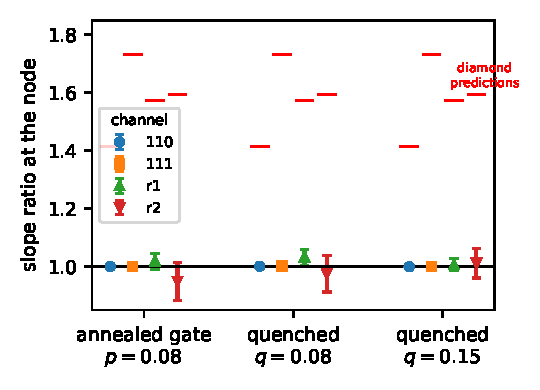
\includegraphics[width=\columnwidth]{figs/cone_ratios.pdf}
\caption{Slope ratios at the node, gate and quenched rows at each $q$,
against the factorized-transport (diamond) prediction. Error bars are
leave-one-block-out jackknives over ten independent medium blocks with
the same-$q$ gate-row systematic added in quadrature. \evX{}}
\label{fig:cone}
\end{figure}

Results (Fig.~\ref{fig:cone}): each measured $q$ carries its own annealed
gate row, and the gate rows reproduce the exact operator (cubic-channel
ratios within $10^{-3}$ of unity at $q=0.08$ and within $6\times10^{-3}$
at $q=0.15$; off-symmetry channels within their own statistics; node
modulus $0.622$ vs $0.620$ at $q=0.08$), with the per-channel deviations
recorded as systematics. On the quenched vacuum at
$q=0.08$ the slope ratios are $r_{110}=1.001\pm0.002$,
$r_{111}=1.002\pm0.002$, $r_{\mathrm a}=1.032\pm0.027$ and
$r_{\mathrm b}=0.976\pm0.064$ for the two off-symmetry directions. The
factorized-transport prediction is excluded in every channel: the weakest
exclusion---by construction the off-symmetry channel with the fewest
orbit members---sits $9.7$ of its error bars from the diamond value
($9.7\sigma$ under a Gaussian reading), and the cubic channels sit more
than $200$ error-bar widths away. The $q=0.15$ row is a consistency
check, not a second headline: its ratios ($r_{110}=1.000\pm0.004$,
$r_{111}=1.000\pm0.006$, $r_{\mathrm a}=1.007\pm0.053$,
$r_{\mathrm b}=1.012\pm0.076$; errors dominated by the $q=0.15$ gate
row's own systematics) exclude the diamond with weakest channel at
$7.7$ widths. Absolute speeds carry the full medium-ensemble
uncertainty, $v(0.08)=1.03\pm0.18$, consistent with the exact $1.18$; at
$q=0.15$ the $\delta k\to0$ extrapolation of the absolute scale is
curvature-dominated (linearity residual $0.30$) and only the ratios are
quoted. The quenched node parameters themselves shift from the annealed
closed forms---$|\lambda_0|$ by $+2.8\%$ and $\omega_0$ by $+8.6\%$ at
$q=0.08$---of which the gate row's own instrumental offsets account for
$+0.3\%$ and $+2.3\%$; the remainder is a property of the quenched
medium (re-read correlations), not of the instrument. \evX{}

\subsection{Helicity residues}

At the node the effective generators $h_a$ on the doublet satisfy the exact
Clifford algebra $\{h_a,h_b\}=2v^2\delta_{ab}$; because the node frame of
the damped (non-normal) operator is not unitary, the Pauli coefficients of
$h_a$ are complex with \emph{bilinear} orthogonality
$R^TR=v^2\openone$ ($R\in O(3,\mathbb C)$), and
$\det R=-v^3$ exactly: chirality $\chi=-1$ \evM{}. The split branches'
spectral projectors equal the helicity projectors
$\tfrac12(\openone\pm n\cdot\sigma)$, $n=Ru/\sqrt{(Ru)\!\cdot\!(Ru)}$.
Measured on the quenched vacuum (the 26 directions of the cubic
$\{100\}/\{110\}/\{111\}$ stars at each of the three---by
$\pi$-periodicity identical---corner representatives; gate row passed):
helicity-map bilinear isotropy
$0.020\pm0.010\,(\mathrm{stat})\pm0.048\,(\mathrm{syst})$---the
systematic being the annealed gate row's own return, $0.048\pm0.014$,
for the identical estimator---chirality $-1$ (stable under every
jackknife resampling), pointwise
$|1-n\cdot n_{\rm exact}|$ of mean $0.010\pm0.002$ \evX{}. (The residue
projectors are rank one by construction of the spectral estimator, so
``purity'' is not reported as a measurement.) One convention is essential for eigenvector work: the
$e^{-ik\cdot x}$ Fourier contraction estimates $U(-k)=\bar U(k)$, whose
upper-half eigenvectors belong to the opposite-helicity conjugate doublet;
residue measurements must use $e^{+ik\cdot x}$.

\section{Exact quantum mechanics}
\label{sec:exactqm}

\subsection{Complex structure}

Let $P$ be the lifted carrier particle--hole conjugation, the Majorana
string $\prod_i(a_i+a_i^\dagger)$ over carrier modes. In the segregated
ordering, $P$ is real orthogonal with $P^2=+1$ (carrier mode number
$M=4L^3\equiv0 \bmod 4$), and
\begin{equation}
[\hat S, P]=0
\end{equation}
\emph{exactly, including all lift signs}: verified on the complete Fock
space of a ring substrate, and in genuine three-dimensional geometry on the
sector pairs $\{0,1,2,M{-}2,M{-}1,M\}$ (particle--hole duality maps the
deep sectors to one- and two-hole problems), per layer and full cycle at
$L=2,3$ \evM{}. With the grading $\eta=\mathrm{sign}(N_c-M/2)$---conserved
by every layer, odd under $P$, and size independent away from half
filling---define
\begin{equation}
K=\mathrm{diag}(\eta), \qquad I = P\,\mathrm{diag}(\eta).
\end{equation}
Then $K^2=1$, $I^2=-1$, $\{K,I\}=0$, $I$ antisymmetric, and $[\hat S,I]=0$;
with multiplication $(\alpha+i\beta)q:=\alpha q+\beta Iq$ and the induced
Hermitian form, $\hat S$ is a unitary operator on a complex Hilbert
space~\cite{Wetterich2022}: the automaton's quantum mechanics is exact
\evM{}. On the substrate the construction extends to the half-filled sector
by an explicit orbit-wise grading; in three dimensions no size-independent
grading of the half-filled sector was found and the question is left open.
All physical sectors (vacuum plus finitely many carriers) are covered
rigorously at every size.

\subsection{Bridge to the spectral analysis}

The complex structure above is global (a Majorana string), and the
spectral results of Sec.~\ref{sec:spectrum} use the ordinary Fourier $i$.
These are the same quantum mechanics, by an explicit intertwiner: the map
$\Phi(u+iv)=u\oplus(-Pv)$ is a complex-linear isomorphism from the
complexified one-particle sector with the Fourier $i$ onto the
$(V_1\oplus V_{M-1},I)$ eigensector of the automaton's Hilbert space,
intertwining the dynamics (this is exactly $[\hat S,P]=0$ restricted to
the sector) and the Hermitian forms. Consequently the measured propagator
\emph{is} an $I$-Hermitian matrix element, every $\pm\omega$ conjugate
pair of the Fourier analysis appears once as a particle and once as an
antiparticle in the $(K,I)$ picture, and the chirality bookkeeping of
Sec.~\ref{sec:spectrum} is the particle/antiparticle structure of a
single Weyl node. Machine-checked in three dimensions: the intertwining
identities hold exactly and the form isometry to $3\times10^{-15}$
\evP{}, \evM{}. What remains genuinely distinct is the damping: the
in-state reduced dynamics is a contraction (the chord), and only the
two-boundary amplitudes of Sec.~\ref{sec:damping} are unitary (the arc);
the bridge identifies the kinematics, not the dissipative structure.

\subsection{Grassmann action}

The local factors and actions of all blocks are extracted mechanically in
exact rational arithmetic by the pipeline of
Ref.~\cite{Wetterich2022}, Eqs.~(51)--(58), validated term by term on the
interaction block of that reference%
\footnote{The validation surfaced one typographical error in
Ref.~\cite{Wetterich2022b}: the coefficient of the top monomial in the
closed-form interaction action, Eq.~(38) there (source label CS9;
equation number confirmed by compiling the arXiv source), must be $-2$,
not $-1$; the printed value fails the defining relation $e^{-L}=K$ at
that single monomial.}. For the coincube conversion blocks the physical (Givens-lift)
gauge yields an axis-universal action: 40 terms with identical degree
structure for all three axes; the quadratic part is the signed-swap
bilinear of $C_a$ plus the environment transport term, and the
environment control appears as quartic and higher couplings between the
channel bilinears and $e^\prime\tilde e$ \evM{}.

\section{Mass: inversion doubling}
\label{sec:mass}

Doubling the coin with a mass bit $b_m$ whose value \emph{reverses all
direction assignments}, $d^{(8)}_a=d_a\otimes\mathrm{diag}(1,-1)$, with
conversions blind to $b_m$, places two opposite-chirality copies of the
node at the same momentum and frequency (the $b_m{=}1$ sector is the
spatial-inversion image; sector chiralities $\mp1$ verified) \evM{}. The
alternative doubling $C_a\otimes Z$ fails for cause: $-C_a$ generates the
opposite triple orientation, which is the \emph{other} corner frequency
family, so the two sectors share no node. A mass layer
$M=(1-q_m)\openone+q_m C_m$ with $C_m=\openone_4\otimes XZ$ (a
$b_m$-flipping controlled Givens, driven by a fourth environment field of
density $q_m$) couples the chiralities. Two operator identities carry the
sector \evP{}: $U(k)=(\openone\otimes R_m)[U_4(k)\oplus U_4(-k)]$ and, at
the node, $U(0)=U_4(0)\otimes M_2$ with $M_2$ a scaled rotation of the mass
bit; hence the gap is \emph{exactly}
\begin{equation}
2m \;=\; 2\arctan\!\frac{q_m}{1-q_m},
\label{eq:massgap}
\end{equation}
independent of $q$, with the multiplet center unshifted; frequencies add
angles as in a telegraph process, and $m=q_m+O(q_m^2)$ recovers the Kac
form~\cite{Kac}. On the node space the generators obey the full Dirac--Clifford
algebra $\{h_a,h_b\}=2v^2\delta_{ab}$, $\{h_a,\beta\}=0$, $\beta^2=1$,
identically in $q$ \evP{}, so
$\omega=\omega_c\pm\sqrt{m^2+v^2k^2}$ at leading order with the exact
finite-$k$ composition law
$\cos(\omega-\omega_c)=\cos m\,\cos\varphi_{\rm massless}(k)$.
No real Dirac mass exists at four components: the anticommutant of the
quaternionic triple $\{C_a\}$ in $M_4(\mathbb R)$ is zero-dimensional
\evM{} (for a $\mathrm{Cl}(3,0)$ triple with squares $+1$ the
anticommutant is two-dimensional with strictly negative squares---
wrong-sign masses only); eight components are minimal, as realized here.

The census of Sec.~\ref{sec:census} extends to the massive model: the
corner and all three half-point nodes acquire the \emph{identical} gap
$2\arctan[q_m/(1-q_m)]$ (deviation below $10^{-12}$), the half-points
becoming additional anisotropic Dirac species, while the nodal lines
split only weakly ($2m/9.8$ at $(0.7,\pi/2,\pi/2)$ for $q=0.08$; $2m/5.0$
at $q=0.15$), leaving sub-gap remnant states inside the Dirac gap \evM{}.

\begin{figure*}[!t]
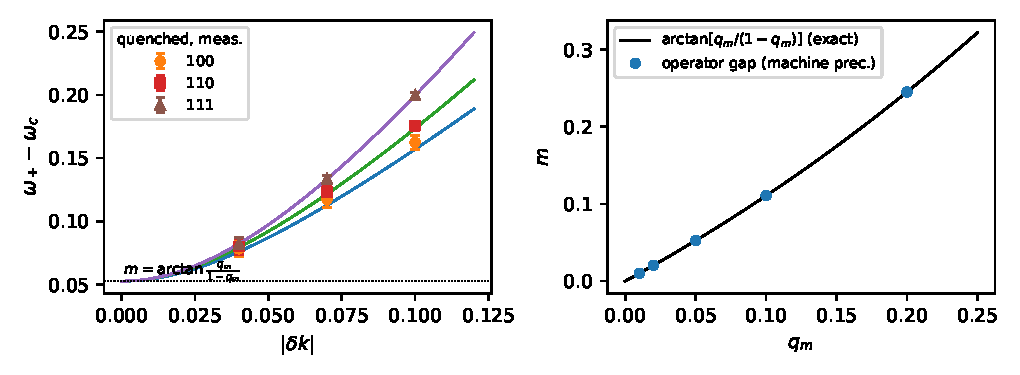
\includegraphics[width=0.85\textwidth]{figs/mass.pdf}
\caption{Left: measured quenched massive dispersion (markers,
$q=0.08,\ q_m=0.05$) on the exact operator branches (lines); the family
ordering of the curvatures is the exact model's. Right: the operator gap
against the closed form, Eq.~(\ref{eq:massgap}), agreeing to machine
precision. \evX{}, \evP{}}
\label{fig:mass}
\end{figure*}

Measured on the quenched vacuum with the gated eight-launch instrument
(Fig.~\ref{fig:mass}): the gap is
$m=0.0547\pm0.0038$ against the closed form $0.0526$ (the gate row's own
estimator carries a $+1.7\sigma$ pair-splitting bias at the same setting,
recorded as a systematic), the multiplet center is
$\omega_c=0.3182\pm0.0027$, and the dispersion lies on the exact
operator branches with a maximum pull of $1.0$ jackknife errors over all
nine (family, $\delta k$) points---machine-asserted from the committed
run output---with the family ordering of the curvatures that the exact
model prescribes \evX{}.

\section{Interaction}
\label{sec:interaction}

For fixed media the multi-carrier sector is exactly determinantal
(Sec.~\ref{sec:coincube}), so genuine interaction requires
\emph{back-reaction}. The imprint layer L4 acts once per cycle: at sites
where an autonomous four-valued field fires (pair $(xy)$, $(yz)$ or $(zx)$
with probability $g/3$ each) \emph{and} the site's carrier fermion parity
is odd, the selected two environment species at that site are swapped.
The imprint field is autonomous in the same sense as the media: its
randomness lives in the initial product measure only (value $0$ with
probability $1-g$), and it evolves by legal deterministic pair-swap
streaming with the axis rotating per cycle. A per-cycle resampled field
would be a stochastic rule---an annealed approximation, not an
automaton---and is not used.
Three design facts are load bearing. (i)~A fixed swap pair breaks cubic
symmetry at $O(g)$ (anisotropic node corrections at $10\sigma$); the
rotating $C_3$-covariant triple is protected at all orders \evX{}, \evP{}.
(ii)~Parity control (not occupancy) is particle--hole even, so the complex
structure of Sec.~\ref{sec:exactqm} survives at $g>0$ unchanged \evM{}.
(iii)~The lift gauge of the imprint is \emph{physical}: the permutation
lift ($|11\rangle\to-|11\rangle$) and the Givens lift differ by a
parity-controlled sign with identical classical dynamics but per-event
coherent deficits $2q^2$ versus $2q(1-q)$; we fix the permutation lift
(minimal decoherence) \evM{}.

Certificates. The connected two-particle correlator
$C_2=G_2-\det G_1$ is nonzero already at $g=0$---the model is an
interacting carrier--environment theory at the correlator level, with
free-fermion structure only per medium realization---so the interaction
certificate is differential: $\Delta C_2(g)=C_2(g)-C_2(0)$ vanishes
identically at $g=0$ and switches on linearly,
$\Delta C_2/g\simeq0.35$ on the exact substrate \evM{}. A control-variant
experiment (occupancy-controlled imprint, used only as an instrument
control) separates the parity-blocking contact artifact: $2$--$3\%$ of the
signal \evM{}.

Survival. The parity control makes the vacuum imprint-transparent, so the
one-sided ensemble amplitude stays closed:
$U_g(k)=(1-2gq^2)\,U(k)$ at annealed order---the cone, residues and mass
are untouched, at a damping cost $\Gamma_{\rm int}=2q^2g$ per cycle
($\sim0.3\%$ of the free width at $q=0.08$, $g=0.1$) \evP{}. The identity
that anchors the instrument: the media-ensemble walker average \emph{equals}
the canonical coherent-vacuum correlator exactly \evM{}. Quenched
three-dimensional measurement with paired common-noise walkers (the
instrument passes an exact known-answer gate: at $g=0$ the paired
branches agree bit for bit): the law is confirmed at the first cycle to
$7\times10^{-4}$ absolute (worst coupling, $g=0.6$), with first-cycle
momentum spread below $10^{-4}$ across the node region, so isotropy
survives interaction by measurement as well; over six cycles the paired
ratio stays momentum independent to $\le1.2\%$ wherever the amplitude
gate retains all six probe momenta (at one intermediate cycle the gate
retains a single momentum and $k$-independence is not claimed there);
beyond leading order the re-read (recross) channel partially
\emph{recoheres} the amplitude, so the asymptotic $\Gamma_{\rm int}$ is
bounded above by the law \evX{}.

\section{Damping: a theorem and its unitary completion}
\label{sec:damping}

\begin{figure}[!htb]
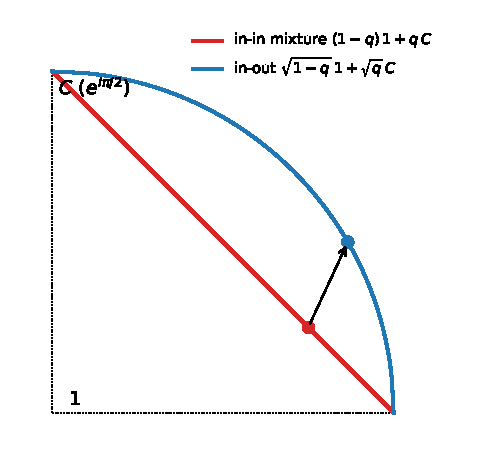
\includegraphics[width=0.75\columnwidth]{figs/chord_arc.pdf}
\caption{Geometry of Theorem~\ref{thm:qbound}. Probabilistic (in-state)
mixtures of the identity and a quaternion unit lie on the chord (damped
interior); the two-boundary weights lie on the unitary arc. The isotropic
node splitting is a property of the whole family
$E_a(\alpha\openone+\beta C_a)$, for all weights.}
\label{fig:chord}
\end{figure}

The dressed quasiparticle of the classical in-state observable is damped:
$\Gamma(q)=-3\ln[(1-q)^2+q^2]$ exactly, with quality factor
$Q=\omega_0/\Gamma$ between $0.60$ and $0.90$ across the working range,
\emph{not} improving as $q\to0$ inside the relativistic window (both
$\omega_0$ and $\Gamma$ scale with $q$). Proposition~\ref{prop:factor}
states precisely what kind of damping this is: at annealed order
$U(k)=\rho^6V(k)$ with $V(k)$ unitary, so $\Gamma=-3\ln\rho^2$ is a
mode-blind, $k$-independent \emph{interference-visibility} decay---every
coherent mode decays at the same rate relative to the conserved
probability sector, whose Perron eigenvalue in the doubled description
remains exactly $1$. It is not a broadening of the node relative to any
other mode. Nor is it a removable normalization: the in-state
normalization is fixed by probability conservation, and the
visibility-to-probability ratio is physical. All \emph{mode-selective}
decoherence resides in the quenched re-read corrections, quantified at
the end of this section. That the visibility decay cannot be tuned away
is structural:

\begin{theorem}[Q-pinning, quaternionic event class]\label{thm:qbound}
Let every conversion event lie in the quaternionic set
$\mathbb R\cdot Q_8=\{\pm\openone,\pm C_x,\pm C_y,\pm C_z\}$. Then for
any product of convex mixtures of events---non-commuting factors and
arbitrarily correlated weights included---every eigenvalue $\lambda$ of
the composite obeys
$\mathrm{dist}(\arg\lambda,(\pi/2)\mathbb Z)\le\kappa\,(-\ln|\lambda|)$
with $\kappa=\pi/(2\ln2)$ exactly. Moreover, under three further
hypotheses---(i) events in $\mathbb R\cdot Q_8$ controlled by
per-engagement reads of binary media; (ii) the coincube read geometry,
in which the two same-axis engagements read lattice-adjacent sites with
both offsets realized across coin branches; (iii) a deterministic
environment rule with randomness confined to the initial measure---an
isotropic node forces $\Gamma>0$: node unitarity requires an
almost-surely deterministic conversion word, the only
translation-invariant binary media with deterministic window counts are
the crystals, and both crystal classes destroy the cone. \evP{}
\end{theorem}

The restriction to the quaternionic class is necessary, not stylistic:
for transposition events on three or more modes (eigenvalue angles
$\{0,\pi\}$) products of mixtures develop three-cycle eigenvalues near
$e^{2\pi i/3}$, and the phase-per-decay ratio is unbounded ($4.95$ at
mixing weight $\epsilon=0.05$, $131$ at $\epsilon=0.002$); for event
sets with finest eigenvalue angle $2\pi/\ell$ the constant grows as
$\kappa(\ell)\to2\ell/\pi$ \evM{}. The bound is a statement about the
quaternionic class, degrading linearly with coin refinement. In these
terms the theorem reads: no legal in-state automaton of this class can
advance any mode's interference phase by more than $\kappa$ radians per
$e$-fold of visibility decay, and ``an isotropic node forces
$\Gamma>0$'' asserts a nonzero uniform visibility decay, not a node
width.

The idealized ordered-dimer environment does achieve the commutator-limited
decoherence $\Gamma=k^2/2$ per event---the branch-remerging mechanism is
real---but its velocity fan collapses to the diamond: within the legal
class, cone and in-state unitarity are mutually exclusive.

The completion is the two-boundary object. The isotropic node splitting
holds for the whole family $E_a(\alpha\openone+\beta C_a)$, and by the
identity of Proposition~\ref{prop:factor},
$T^\dagger T=(\alpha^2+\beta^2)\openone$ for every real weight pair (the
two-boundary walk is the $\alpha^2+\beta^2=1$ member of the same
family): \emph{every} product final boundary
$(w_0,w_1)$ yields zero relative damping and an isotropic node, landing on
the unitary arc at $s^2=w_1^2q/[w_0^2(1-q)+w_1^2q]$ \evP{}. The
completions thus form a one-parameter family; in-state weights $(1-q,q)$
lie on the damped chord, and the square-root point
$(\sqrt{1-q},\sqrt q)$ (Fig.~\ref{fig:chord}) is selected uniquely as
the only \emph{medium-blind} boundary---the only choice invariant under
flipping the environment bits ($w_0^2=w_1^2$) \evP{}. Numerically: all
$|\lambda|=1$ to $4\times10^{-16}$ with slope isotropy asserted below
$10^{-3}$ and $\omega_0$ tunable at the $\sqrt q$ scale \evM{}. In
quenched three dimensions the fresh-read law is exact at the first cycle
(coherent path enumeration, no sampling), with growing recoherent re-read
corrections thereafter ($11$--$25\%$ by three cycles at $q=0.08$); the
long-time pole structure of the quenched two-boundary object is open.
\evM{}

\section{Discussion}
\label{sec:discussion}

Under the strictest single-fermion contract, the free-fermion sector of the
three-dimensional problem posed in Ref.~\cite{Wetterich2022} is solved: a
legal probabilistic cellular automaton whose dynamics is exactly unitary
quantum mechanics and whose single-carrier excitation on a clustering
product vacuum is an isotropic Weyl fermion---dispersion and spinor
residues---extendable to a massive Dirac fermion with an exact tunable
mass, and to a certified media-mediated interaction under which the free
spectrum survives at leading order. Every closed form is verified against
the operators it describes, and every measurement runs behind a
known-answer gate. The solution is a lattice fermion in the standard
sense: the census of Sec.~\ref{sec:census} places its partner species at
displaced momenta and quasienergies rather than removing them.

The precise open problems are: (i) the half-filled carrier sector of the
complex-structure construction in three dimensions; (ii) the long-time
behavior of the quenched two-boundary propagator (re-read resummation);
(iii) the continuum limit and the fate of Lorentz symmetry beyond the
leading cone, including interaction corrections beyond the scalar law; and
(iv) multi-carrier physics beyond the contact terms already present in the
extracted quartic action; and (v) the physics of the sub-gap nodal-line
remnants of the massive census. The damping of the in-state quasiparticle
is not on this list: it is an exact, mode-blind prediction of the
construction (Proposition~\ref{prop:factor}), bounded by
Theorem~\ref{thm:qbound}, and absent from the two-boundary amplitude.

\begin{acknowledgments}
Derivations, code, verification protocols and drafts were prepared with
substantial assistance from the AI system Claude (Anthropic); all results
were machine-verified as described, and the author takes full
responsibility for the content. The complete verification code and the
manuscript source are available at Ref.~\cite{repo}.
\end{acknowledgments}


\appendix

\section{Proofs}
\label{app:proofs}

\subsection{Theorem \ref{thm:finiteray} (finite rays)}

Let the rule conserve particle number in the one-particle sector. Its
restriction to that sector is a signed permutation of the species basis
composed with site shifts, so the Bloch operator has matrix elements
$S(k)_{\alpha\beta}=s_{\alpha\beta}e^{ik\cdot d_{\alpha\beta}}$ with, by
the unique-jump property, exactly one nonzero entry in each row and column:
a monomial matrix. Its characteristic polynomial factorizes over the cycles
of the underlying permutation; a cycle of length $\ell$, accumulated
displacement $D$ and sign $\sigma$ contributes
$\lambda^\ell=\sigma\,e^{ik\cdot D}$, i.e.
$\omega_m(k)=(k\cdot D+\arg\sigma+2\pi m)/\ell$: every branch is exactly
linear with group velocity $D/\ell$, drawn from the finite set of cycle
data. A cone $\omega=v|k|$ requires a two-sphere of group velocities. The
deviation of any finite ray set from a sphere is scale invariant, so no
continuum limit removes it; and a periodic cycle of rotated rules is again
unique-jump (products of signed permutations are signed permutations), so
the theorem applies to the composite rule. \hfill$\square$

\subsection{Theorem \ref{thm:ntwo} (two-component states)}

Three ingredients. (i) \emph{Algebraic ceiling.} On
$\mathfrak{sl}_2(\mathbb R)$ every element satisfies
$X^2=-\det(X)\openone$ and anticommuting elements are orthogonal in the
polarization of $\det$; in the basis $\{X,Z,XZ\}$ the squares are
$+\openone,+\openone,-\openone$, so the form has signature $(2,1)$ and no
real two-dimensional representation of $\mathrm{Cl}(3,0)$ exists.
(ii) \emph{Generic weights.} A symbolic orthogonality lemma for the
mixture families shows that a degenerate propagating pair at any momentum
requires $(1-p)^2=p^2$ for rotation coins, is impossible for reflection
coins, and degenerates for diagonal coins: a linear node forces
$U(k_0)=\lambda_0\openone$, the splitting generators are conjugated
involutions with automatically scalar anticommutators ($2\times2$
Cayley--Hamilton), and the required bilinear orthogonality gives
$T_{00}T_{11}=-T_{01}T_{10}$. For the blocked two-origin cycles, an
exhaustive sweep (all 512 sign/direction tables per placement, both
engagement patterns, $p\in\{0.15,0.25,0.35,0.5\}$, multistart continuous
momentum search) establishes strictly positive anisotropy floors at
generic $p$, with per-sector assertions.
(iii) \emph{The fine-tuned points.} At the singular weight $p=\tfrac12$
the single-origin placement has $U(k_0)$ scalar at
$k_0=(\tfrac{3\pi}4,\tfrac{3\pi}4,-\tfrac\pi4)$ (and its symmetry
images), and the three effective generators form an exact complex
Clifford triple, giving $\omega=\pi\pm|\delta k|$: an isotropic node with
every parameter frozen and $\Gamma=\tfrac32\ln2$ at the chord midpoint.
In the blocked placements, branch continuation in $p$ (warm-started exact
scalar solves with probe-radius-extrapolated anisotropy) locates
codimension-one transversal zeros of the single remaining Gram condition
at $p^*=0.3300$ (additive placement,
$k_0/\pi=\pm(0.916,0.916,-0.916)$, $|\lambda_0|=0.1736$) and
$p^*=0.3204$ (multiplicative, $|\lambda_0|=0.1799$), both with
$\omega_0=\pi$ and $\chi=-1$: isolated tuned nodes, not parameter
families. All parts are machine-checked, the sweep exhaustively.
\hfill$\square$

\subsection{The mass identity, Eq.~(\ref{eq:massgap})}

At $k=0$ the momentum factors are the identity, so the direction reversal
that distinguishes the two $b_m$ sectors is invisible and the axis layers
act as $U_4(0)\otimes\openone_2$. The mass layer acts on the $b_m$ factor
alone: $M_2=(1-q_m)\openone+q_m XZ$, a real multiple of a rotation with
$\arg$-eigenvalues $\pm\arctan[q_m/(1-q_m)]$ and modulus
$\sqrt{(1-q_m)^2+q_m^2}$. Hence
$U(0)=U_4(0)\otimes M_2$: the spectrum is the product set, frequencies add
angles, the multiplet center is unshifted, and the gap is exactly
$2\arctan[q_m/(1-q_m)]$, independent of $q$. \hfill$\square$

\subsection{Theorem \ref{thm:qbound} (Q-pinning)}

Any product of convex mixtures of the event set is itself a convex mixture
over the quaternion group $Q_8$ (the product measure is the convolution on
the group, so correlations between events are automatically included). In
the quaternion representation such a mixture is
$T=w\openone+x C_x+y C_y+z C_z$ with $|w|+\lVert(x,y,z)\rVert_1\le1$,
and its eigenvalues are $w\pm i\lVert(x,y,z)\rVert_2$. Since
$\lVert\cdot\rVert_2\le\lVert\cdot\rVert_1$, every eigenvalue lies
inside the convex hull of the chords between adjacent fourth roots of
unity; on the extremal chord $1\to i$, $\lambda=(1-t)+it$ has
$\arg\lambda/(-\ln|\lambda|)$ maximized at the midpoint $t=\tfrac12$,
where it equals $\pi/(2\ln2)$. This bounds
$\mathrm{dist}(\arg\lambda,(\pi/2)\mathbb Z)\le\kappa\Gamma$ for
arbitrary, non-commuting products---the full statement of the theorem.
The group closure is the load-bearing hypothesis: outside
$\mathbb R\cdot Q_8$ (already for transposition events on three modes)
products of mixtures leave the span of the event set, three-cycle
eigenvalues appear, and the measured phase-per-decay ratios grow without
bound, as reported in the main text.
For the second statement (under hypotheses (i)--(iii), the read-window
structure being hypothesis (ii)): unitarity of the node eigenvalue
requires the conversion count $N$ (mod 4) along a read window to be
deterministic, by
$|\mathbb E[i^N]|^2=(p_0-p_2)^2+(p_1-p_3)^2\le1$ with equality only at a
vertex; translation-invariant binary media with deterministic window
counts are exactly the two uniform and two staggered crystals (enumerated
exactly on rings); and the deterministic-word cycles' spectra are computed
explicitly and are never isotropic. Machine checks accompany every step,
including randomized non-commuting products. \hfill$\square$

\section{Verification protocols}
\label{app:verify}

Every claim tagged \evM{} is an assertion in a runnable script; the
tolerances quoted below are the assertion thresholds, and each script is
self-checking (it fails loudly rather than reporting).

\emph{Layer lifts.} The conversion layer is verified densely on the
one-site Fock space (32 states): the controlled double Givens is a signed
permutation of the basis, unitary, commutes with fermion parity, is the
identity on the empty control sector, has single-particle matrix equal to
the signed-swap block of $C_a$, satisfies $G^2=-\openone$ on the
one-particle sector, and maps the doubly occupied pair to $+$ itself
(determinant one), for all three axes, to $10^{-12}$.

\emph{Composite sign coherence.} The full cycle is built as a signed
permutation of the many-body basis from the stored per-layer sign rules
(spectator Jordan--Wigner strings for conversions; inversion and wrap
parity for translations), in the segregated mode ordering. For random
environment configurations the zero-, one- and two-particle sectors are
extracted and compared: the one-particle sector must equal the stated rule
and the two-particle sector the antisymmetrized square $\Lambda^2M_1$,
exactly. This holds on the full Fock space of a ring substrate ($2^{15}$
states) and in three-dimensional geometry at $L=2$ (496 pair states) and
$L=3$ (5778 pair states). Mutation controls certify sensitivity: deleting
the spectator string produces $8/496$ mismatches; deleting translation
parity produces $2772/5778$ at $L=3$ (counts are specific to the
committed environment draw) and---the recorded caveat---$0$ at
$L=2$, where two sub-steps per axis make net crossings even.

\emph{Complex structure.} $P$ is applied as the Majorana string with its
Jordan--Wigner signs; $[\hat S,P]=0$ is checked as an identity of signed
permutations (both orderings byte-identical), on the full substrate Fock
space and, in three dimensions, on the sectors
$\{0,1,2,M-2,M-1,M\}$ using particle--hole duality to reduce the deep
sectors to one- and two-hole problems; per layer and for the full cycle.
The unitarity of the complex picture is verified as invariance of the
induced Hermitian form on random vectors to $10^{-9}$.

\emph{Grassmann extraction.} Local factors are built from the block tables
over exact rationals; $e^{-L}=K$ is asserted exactly before any action is
reported, and the inverse map $K\to(\text{perm},\text{signs})$ must
round-trip. The pipeline is validated term by term against the closed-form
interaction action of Ref.~\cite{Wetterich2022}.

Table~\ref{tab:claims} maps each principal claim to its verification
script in Ref.~\cite{repo}.

\begin{table}[!htb]
\caption{Principal claims and their verification scripts (all
self-asserting; in \texttt{scripts/} of Ref.~\cite{repo} unless noted).}
\label{tab:claims}
\begin{ruledtabular}
\footnotesize
\begin{tabular}{ll}
finite-ray tests & \texttt{tests/test\_finite\_ray\_theorem}\\
$v(q)$ dressing law & \texttt{theory\_linear\_law}\\
Abelian-gauge diamond & \texttt{w2\_scalar\_gauges}\\
coin scans ($n=2,4$) & \texttt{w3\_transfer\_scan}\\
annealed cone & \texttt{w3\_cone\_verify}, \texttt{theory\_real\_cone}\\
lift certificates & \texttt{w3c\_lift\_check}, \texttt{w3c\_composite\_check}\\
3D sector certificates & \texttt{theory\_3d\_certs}\\
quenched cone (gated) & \texttt{w3c\_corner}\\
census; factorization & \texttt{spectrum\_census}\\
two-component taxonomy (Thm~\ref{thm:ntwo}) & \texttt{theory\_redteam}\\
helicity residues & \texttt{w4\_helicity\_exact}, \texttt{w4\_helicity}\\
complex structure & \texttt{e1\_complex\_structure}, \texttt{e1\_interacting}\\
Grassmann actions & \texttt{e2\_coincube\_actions}\\
mass sector & \texttt{m8\_mass\_exact}, \texttt{m8\_corner}, \texttt{theory\_mass}\\
massive dispersion pulls & \texttt{m8\_pulls}\\
interaction & \texttt{i2\_connected}, \texttt{i2\_split}, \texttt{i3\_quenched3d}\\
imprint-field dynamics & \texttt{theory\_interaction}\\
Q-pinning; in--out & \texttt{theory\_q\_bound}, \texttt{a\_inout}, \texttt{a\_inout\_3d}
\end{tabular}
\end{ruledtabular}
\end{table}

\section{Measurement pipeline}
\label{app:instrument}

All \evX{} results use one instrument family. The object is the exact
per-medium single-particle signed field (the single-carrier sector is
linear in the field for fixed media, so this is walker-exact with infinite
walkers), averaged over $R$ media; the media-ensemble average provably
equals the canonical coherent-vacuum correlator.

\emph{Bloch-matrix estimation.} All $n$ basis launches are evolved, giving
the full $n\times n$ propagator series $G(t,k)$; the one-cycle operator is
fit by least squares, $\hat U(k)=G_{t+1}G_t^+$ over a post-transient
window. Momenta are probed off the lattice grid by direct phase
contraction, with probe radii inside the node's measured linear range.

\emph{Pooling.} Naive eigenvalue extraction near a two-fold node is
$\sqrt{\text{noise}}$-ill-conditioned (a noisy nearly defective matrix
splits its double eigenvalue as the square root of the perturbation);
pooling is therefore performed on characteristic-polynomial coefficients
over the symmetry orbit of measurement momenta---a basis-invariant,
\emph{linear} (hence unbiased) average---before rooting. Slopes use
symmetric splittings at two step sizes with $\delta k\to0$ Richardson
extrapolation. Media are accumulated in independent blocks (ten for the
cone instrument, eight for the massive instrument, six for the helicity
instrument) and every final quantity (slope, ratio) is jackknifed at the
end-of-pipeline level over leave-one-block-out samples; the annealed gate
row's deviation from the exact operator is recorded per channel and added
in quadrature as a systematic. Off-symmetry direction families are measured alongside the
cubic stars, and the diamond-exclusion significance is computed in code for
every channel, with the weakest channel quoted.

\emph{Gates.} Every production run carries an annealed known-answer row
through the identical pipeline; a failed gate discards the run. Amplitude
gates exclude momenta near free-beat amplitude nodes for ratio estimators
(shot-noise gating alone is insufficient there). Eigenvector work uses the
$e^{+ik\cdot x}$ contraction (Sec.~\ref{sec:spectrum}). For interaction
ratios, paired common-noise evolution (identical randomness with the
imprint on and off) cancels the medium-ensemble variance, which is
otherwise dominated by low-order conversion caustics. Gate tolerances are
set to catch catastrophic estimator failure (percent scale), not to
certify accuracy; accuracy statements rest on the quoted statistical
errors and the recorded systematics.

\emph{Recorded failure modes.} The following estimator pathologies were
each encountered, diagnosed and firewalled during this program, and are
listed because they generically afflict lattice pole measurements:
(i) $\sqrt{\text{noise}}$ splitting at near-degenerate poles;
(ii) exceptional-point misidentification in damped operators (real double
eigenvalues accepted as propagating nodes);
(iii) through-origin fits across a packet's death into the noise floor;
(iv) ratio blowup at beat-amplitude nodes;
(v) probing outside the (renormalized) linear cone window;
(vi) branch mixing under scalar single-pole estimators at two-fold
degenerate nodes;
(vii) one-dimensional co-streaming substrates, whose companion locking
invalidates absolute calibrations that do transfer in three dimensions.

\section{Closed forms}
\label{app:closedforms}

\begin{table}[!htb]
\caption{Exact expressions of the free and dressed spectra. All are
verified against the operators they describe to at least $10^{-9}$;
$D=\sqrt{1-q}+\sqrt q$.}
\label{tab:closed}
\begin{ruledtabular}
\begin{tabular}{ll}
node modulus & $|\lambda_0|^2=[(1-q)^2+q^2]^6$\\
factorization & $U(k)=\rho^6\,V(k)$, $\rho^2=(1-q)^2+q^2$, $V$ unitary\\
free width & $\Gamma(q)=-3\ln[(1-q)^2+q^2]$\\
cone speed & $v(q)\colon\ 2/\sqrt3 \to 1.207$ (max at $q\simeq0.30$)\\
dressing law (1D) & $v=2|1-2q|$\\
mass gap & $2m=2\arctan[q_m/(1-q_m)]$\\
mass-layer modulus & $\sqrt{(1-q_m)^2+q_m^2}$ per cycle\\
massive dispersion & $\cos(\omega-\omega_c)=\cos m\,\cos\varphi(k)$\\
interaction law & $U_g(k)=(1-2gq^2)\,U(k)$\\
Q-pinning constant & $\kappa=\pi/(2\ln2)=2.2662$\\
in--out transfer & $E_a(k)\,[\sqrt{1-q}\,\openone+\sqrt q\,C_a]/D$,
\ $|\lambda|\equiv1/D$
\end{tabular}
\end{ruledtabular}
\end{table}

Table~\ref{tab:closed} collects the closed forms. Two remarks. The
in--out transfer's uniform modulus $1/D$ per read is a global scalar
(every path reads one bit per sub-step) and is absorbed into wave-function
renormalization; the physical statement is the vanishing of all
\emph{relative} damping. The quality factor of the in-state quasiparticle,
$Q=\omega_0/\Gamma$, rises from $0.60$ to $0.90$ over
$q\in[0.02,0.25]$ and is bounded by $\kappa$ per
Theorem~\ref{thm:qbound}.

\begin{thebibliography}{99}
\bibitem{Wetterich2022} C.~Wetterich,
\emph{Fermionic quantum field theories as probabilistic cellular automata},
Phys.\ Rev.\ D \textbf{105}, 074502 (2022), arXiv:2111.06728.
\bibitem{Wetterich2022b} C.~Wetterich,
\emph{Fermion picture for cellular automata}, arXiv:2203.14081.
\bibitem{Wetterich2022c} C.~Wetterich,
\emph{Cellular automaton for spinor gravity in four dimensions},
arXiv:2211.09002.
\bibitem{KogutSusskind} J.~Kogut and L.~Susskind,
\emph{Hamiltonian formulation of Wilson's lattice gauge theories},
Phys.\ Rev.\ D \textbf{11}, 395 (1975).
\bibitem{NielsenNinomiya} H.~B.~Nielsen and M.~Ninomiya,
\emph{Absence of neutrinos on a lattice}, Nucl.\ Phys.\ B \textbf{185}, 20
(1981).
\bibitem{Kitagawa} T.~Kitagawa, M.~S.~Rudner, E.~Berg, and E.~Demler,
\emph{Exploring topological phases with quantum walks},
Phys.\ Rev.\ A \textbf{82}, 033429 (2010).
\bibitem{Kac} M.~Kac,
\emph{A stochastic model related to the telegrapher's equation},
Rocky Mountain J.\ Math.\ \textbf{4}, 497 (1974).
\bibitem{Wetterich2021NPB} C.~Wetterich,
\emph{Probabilistic cellular automata for interacting fermionic quantum
field theories}, Nucl.\ Phys.\ B \textbf{963}, 115296 (2021),
arXiv:2007.06366.
\bibitem{WetterichPotential} C.~Wetterich,
\emph{Probabilistic cellular automaton for quantum particle in a
potential}, arXiv:2211.17034.
\bibitem{KreuzkampWetterich} A.~Kreuzkamp and C.~Wetterich,
\emph{Quantum systems from random probabilistic automata},
arXiv:2405.09829.
\bibitem{Wetterich2025} C.~Wetterich,
\emph{Complex wave functions, CPT and quantum field theory for classical
generalized Ising models}, arXiv:2505.24392.
\bibitem{tHooft} G.~'t~Hooft,
\emph{The Cellular Automaton Interpretation of Quantum Mechanics},
Fundamental Theories of Physics Vol.~185 (Springer, 2016),
arXiv:1405.1548.
\bibitem{BialynickiBirula} I.~Bia{\l}ynicki-Birula,
\emph{Weyl, Dirac, and Maxwell equations on a lattice as unitary cellular
automata}, Phys.\ Rev.\ D \textbf{49}, 6920 (1994).
\bibitem{Meyer} D.~A.~Meyer,
\emph{From quantum cellular automata to quantum lattice gases},
J.\ Stat.\ Phys.\ \textbf{85}, 551 (1996).
\bibitem{DArianoPerinotti} G.~M.~D'Ariano and P.~Perinotti,
\emph{Derivation of the Dirac equation from principles of information
processing}, Phys.\ Rev.\ A \textbf{90}, 062106 (2014).
\bibitem{BisioDAriano} A.~Bisio, G.~M.~D'Ariano, and P.~Perinotti,
\emph{Simple derivation of the Weyl and Dirac quantum cellular automata},
Phys.\ Rev.\ A \textbf{95}, 062344 (2017).
\bibitem{Arrighi} P.~Arrighi,
\emph{An overview of quantum cellular automata},
Nat.\ Comput.\ \textbf{18}, 885 (2019).
\bibitem{Farrelly} T.~Farrelly,
\emph{A review of quantum cellular automata},
Quantum \textbf{4}, 368 (2020).
\bibitem{MlodinowBrunNoGo} L.~Mlodinow and T.~A.~Brun,
\emph{Quantum field theory from a quantum cellular automaton in one
spatial dimension and a no-go theorem in higher dimensions},
Phys.\ Rev.\ A \textbf{102}, 042211 (2020).
\bibitem{BrunMlodinow2D} T.~A.~Brun and L.~Mlodinow,
\emph{Quantum cellular automata and quantum field theory in two spatial
dimensions}, Phys.\ Rev.\ A \textbf{102}, 062222 (2020).
\bibitem{MlodinowBrun3D} L.~Mlodinow and T.~A.~Brun,
\emph{Fermionic and bosonic quantum field theories from quantum cellular
automata in three spatial dimensions},
Phys.\ Rev.\ A \textbf{103}, 052203 (2021).
\bibitem{Susskind} L.~Susskind,
\emph{Lattice fermions}, Phys.\ Rev.\ D \textbf{16}, 3031 (1977).
\bibitem{DoublingQW} C.~Gupta and A.~J.~Short,
\emph{Fermion doubling in Dirac quantum walks},
Phys.\ Rev.\ A \textbf{114}, 012208 (2026), arXiv:2601.15885.
\bibitem{Bergholtz} E.~J.~Bergholtz, J.~C.~Budich, and F.~K.~Kunst,
\emph{Exceptional topology of non-Hermitian systems},
Rev.\ Mod.\ Phys.\ \textbf{93}, 015005 (2021).
\bibitem{repo} P.~Topa, \emph{coincube: verification code for this
paper}, \url{https://github.com/PiotrTopa/coincube}, tag \texttt{v1.2.0}.
\end{thebibliography}

\end{document}
